\documentclass[11pt,a4paper]{article}
\usepackage[utf8]{inputenc}
\usepackage[margin=1in]{geometry}
\usepackage{graphicx}
\usepackage{booktabs}
\usepackage{tikz}
\usetikzlibrary{shapes.geometric, arrows, positioning, calc}
\usepackage{pgfplots}
\pgfplotsset{compat=1.17}
\usepackage{xcolor}
\usepackage{hyperref}
\usepackage{longtable}

\definecolor{matched}{RGB}{76, 175, 80}
\definecolor{unmatched}{RGB}{244, 67, 54}
\definecolor{stage1}{RGB}{33, 150, 243}
\definecolor{stage2}{RGB}{156, 39, 176}
\definecolor{stage3}{RGB}{255, 152, 0}
\definecolor{stage4}{RGB}{0, 150, 136}

\title{JJM to SHRUG Village Mapping\\Karnataka State}
\author{Data Processing Report}
\date{November 2024}

\begin{document}

\maketitle

\section{Overview}

This document describes the process of mapping Jal Jeevan Mission (JJM) villages in Karnataka to SHRUG (Socioeconomic High-resolution Rural-Urban Geographic) identifiers for linking water infrastructure data with socioeconomic indicators.

\section{Dataset Descriptions}

\subsection{JJM (Jal Jeevan Mission)}
The Jal Jeevan Mission is a Government of India program aimed at providing tap water connections to every rural household. The JJM dataset contains village-level information about water schemes, infrastructure, and coverage.

\begin{itemize}
    \item \textbf{Source:} \url{https://ejalshakti.gov.in/JJM/JJMReports/}
    \item \textbf{Coverage:} Karnataka state, all 31 districts
    \item \textbf{Records:} 26,678 villages
    \item \textbf{Key identifiers:} JJM Village ID (IMIS ID), LGD Village Code
\end{itemize}

\subsection{LGD (Local Government Directory)}
The Local Government Directory is a standardized directory of administrative units maintained by the Government of India. It provides unique codes for states, districts, sub-districts, and villages.

\begin{itemize}
    \item \textbf{Source:} \url{https://lgdirectory.gov.in/}
    \item \textbf{Purpose:} Common identifier linking JJM to SHRUG
    \item \textbf{Key field:} 6-digit LGD Village Code
\end{itemize}

\subsection{SHRUG (Socioeconomic High-resolution Rural-Urban Geographic)}
SHRUG is a geographic dataset linking Indian administrative units over time. It provides consistent village-level identifiers that can be joined with census data, economic surveys, and other datasets.

\begin{itemize}
    \item \textbf{Source:} Development Data Lab
    \item \textbf{Total records:} 596,389 (All India), 27,556 (Karnataka)
    \item \textbf{Key identifier:} SHRID2 (contains embedded LGD code)
    \item \textbf{Reference year:} 2011 Census boundaries
\end{itemize}

\subsection{Karnataka Scheme Details}
Detailed scheme-level data for water projects in Karnataka including costs, implementation status, and household coverage.

\begin{itemize}
    \item \textbf{Records:} 456,712 scheme records
    \item \textbf{Unique villages:} 26,977
    \item \textbf{Key field:} villageid (maps to jjm\_village\_id)
\end{itemize}

\subsection{WPP Details (Water Purification Plants)}
Detailed information about water purification plant installations including location coordinates, specifications, and maintenance status.

\begin{itemize}
    \item \textbf{Records:} 18,323 WPP installations
    \item \textbf{With valid coordinates:} 11,435 (62.4\%)
    \item \textbf{Key fields:} latitude\_clean, longitude\_clean
\end{itemize}

\section{Data Sources Summary}

\begin{table}[h]
\centering
\begin{tabular}{lrp{5cm}}
\toprule
\textbf{Dataset} & \textbf{Records} & \textbf{Description} \\
\midrule
JJM Karnataka & 26,678 & Village-level water scheme data \\
LGD & -- & Local Government Directory codes \\
SHRUG (All India) & 596,389 & Socioeconomic village database \\
SHRUG (Karnataka) & 27,556 & Karnataka subset \\
Scheme Details & 456,712 & Water scheme implementation data \\
WPP Details & 18,323 & Water purification plant data \\
\bottomrule
\end{tabular}
\caption{Data sources and record counts}
\end{table}

\section{Process Flow}

\begin{figure}[h]
\centering
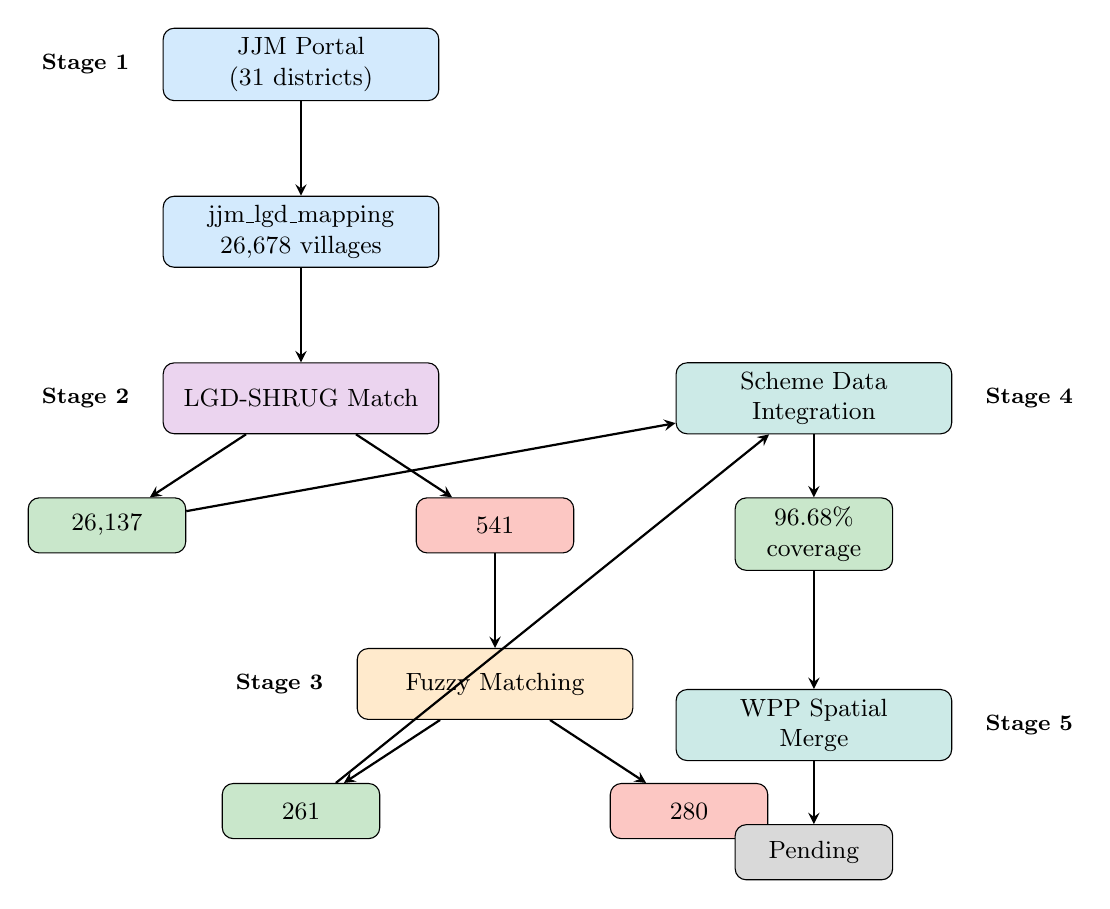
\begin{tikzpicture}[
    node distance=1.2cm,
    box/.style={rectangle, draw, rounded corners, minimum width=3.5cm, minimum height=0.9cm, align=center, fill=white, font=\small},
    result/.style={rectangle, draw, rounded corners, minimum width=2cm, minimum height=0.7cm, align=center, font=\small},
    arrow/.style={->, thick, >=stealth}
]

% Stage 1
\node[box, fill=stage1!20] (source) {JJM Portal\\(31 districts)};
\node[box, fill=stage1!20, below=of source] (jjm) {jjm\_lgd\_mapping\\26,678 villages};

\draw[arrow] (source) -- (jjm);

% Stage 2
\node[box, fill=stage2!20, below=of jjm] (lgdmatch) {LGD-SHRUG Match};
\node[result, fill=matched!30, below left=0.8cm and -0.3cm of lgdmatch] (matched1) {26,137};
\node[result, fill=unmatched!30, below right=0.8cm and -0.3cm of lgdmatch] (unmatched1) {541};

\draw[arrow] (jjm) -- (lgdmatch);
\draw[arrow] (lgdmatch) -- (matched1);
\draw[arrow] (lgdmatch) -- (unmatched1);

% Stage 3
\node[box, fill=stage3!20, below=1.2cm of unmatched1] (fuzzy) {Fuzzy Matching};
\node[result, fill=matched!30, below left=0.8cm and -0.3cm of fuzzy] (matched2) {261};
\node[result, fill=unmatched!30, below right=0.8cm and -0.3cm of fuzzy] (unmatched2) {280};

\draw[arrow] (unmatched1) -- (fuzzy);
\draw[arrow] (fuzzy) -- (matched2);
\draw[arrow] (fuzzy) -- (unmatched2);

% Stage 4
\node[box, fill=stage4!20, right=3cm of lgdmatch] (scheme) {Scheme Data\\Integration};
\node[result, fill=matched!30, below=0.8cm of scheme] (scheme_result) {96.68\%\\coverage};

\draw[arrow] (matched1) -- (scheme);
\draw[arrow] (matched2) -- (scheme);
\draw[arrow] (scheme) -- (scheme_result);

% Stage 5
\node[box, fill=stage4!20, below=1.5cm of scheme_result] (wpp) {WPP Spatial\\Merge};
\node[result, fill=gray!30, below=0.8cm of wpp] (wpp_result) {Pending};

\draw[arrow] (scheme_result) -- (wpp);
\draw[arrow] (wpp) -- (wpp_result);

% Labels
\node[left=0.3cm of source, align=right, font=\footnotesize] {\textbf{Stage 1}};
\node[left=0.3cm of lgdmatch, align=right, font=\footnotesize] {\textbf{Stage 2}};
\node[left=0.3cm of fuzzy, align=right, font=\footnotesize] {\textbf{Stage 3}};
\node[right=0.3cm of scheme, align=left, font=\footnotesize] {\textbf{Stage 4}};
\node[right=0.3cm of wpp, align=left, font=\footnotesize] {\textbf{Stage 5}};

\end{tikzpicture}
\caption{JJM to SHRUG matching pipeline}
\end{figure}

\section{Stage 1: Data Extraction}

\textbf{Script:} \texttt{scripts/01\_combine\_jjm\_lgd\_data.py}\\
\textbf{Output:} \texttt{jjm\_lgd\_mapping\_karnataka.csv}

\subsection{Source}
Downloaded LGD mapping reports from JJM portal for all 31 Karnataka districts. Each district file is an HTML table saved as .xls format.

\subsection{Output Schema}
\begin{table}[h]
\centering
\begin{tabular}{ll}
\toprule
\textbf{Column} & \textbf{Description} \\
\midrule
jjm\_village\_id & JJM Village ID (IMIS ID) \\
jjm\_village & Village name from JJM \\
lgd\_village\_id & LGD Village Code \\
lgd\_village & Village name from LGD \\
jjm\_district & District name \\
jjm\_block & Block/Taluk name \\
jjm\_panchayat & Panchayat name \\
\bottomrule
\end{tabular}
\caption{JJM-LGD mapping schema}
\end{table}

\subsection{Validation Results}
\begin{itemize}
    \item Districts validated: 31/31 (\checkmark)
    \item Total villages: 26,678
    \item Missing LGD IDs: 0
    \item Match rate: 100\%
\end{itemize}

\subsection{Relationship Analysis}
\begin{table}[h]
\centering
\begin{tabular}{lrl}
\toprule
\textbf{Relationship} & \textbf{Count} & \textbf{Status} \\
\midrule
JJM $\rightarrow$ multiple LGD & 0 & \checkmark Clean \\
LGD $\rightarrow$ multiple JJM & 33 & Duplicates \\
\bottomrule
\end{tabular}
\caption{JJM-LGD relationship analysis}
\end{table}

\section{Stage 2: Direct LGD-SHRUG Matching}

\textbf{Script:} \texttt{scripts/02\_direct\_lgd\_shrug\_match.py}\\
\textbf{Input:} \texttt{jjm\_lgd\_mapping\_karnataka.csv}, \texttt{shrid\_loc\_names.csv}\\
\textbf{Output:} \texttt{jjm\_to\_shrug\_direct\_mapping.csv}, \texttt{jjm\_lgd\_to\_shrid\_unmatched.csv}

Exact match on \texttt{lgd\_village\_id} between JJM and SHRUG data. The SHRID2 identifier contains the LGD code in its last 6 digits.

\subsection{Results}

\begin{figure}[h]
\centering
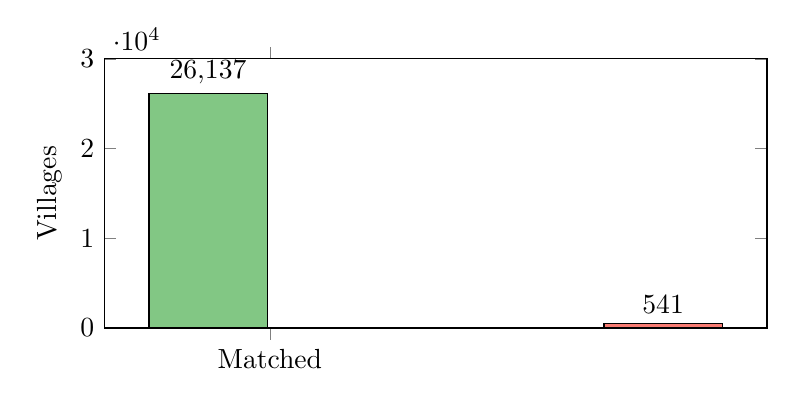
\begin{tikzpicture}
\begin{axis}[
    ybar,
    bar width=1.5cm,
    width=10cm,
    height=5cm,
    ylabel={Villages},
    symbolic x coords={Matched, Unmatched},
    xtick=data,
    nodes near coords,
    nodes near coords align={vertical},
    ymin=0,
    ymax=30000,
    enlarge x limits=0.5,
]
\addplot[fill=matched!70] coordinates {(Matched, 26137)};
\addplot[fill=unmatched!70] coordinates {(Unmatched, 541)};
\end{axis}
\end{tikzpicture}
\caption{Stage 2: Direct LGD matching results}
\end{figure}

\begin{table}[h]
\centering
\begin{tabular}{lrr}
\toprule
\textbf{Status} & \textbf{Count} & \textbf{Percentage} \\
\midrule
Matched & 26,137 & 97.97\% \\
Unmatched & 541 & 2.03\% \\
\midrule
\textbf{Total} & \textbf{26,678} & \textbf{100\%} \\
\bottomrule
\end{tabular}
\caption{Direct matching results}
\end{table}

\subsection{Quality Issues: Duplicate LGD Mappings}

33 LGD codes have multiple JJM entries:
\begin{itemize}
    \item 27 are case variations of the same village
    \item 6 are actual conflicts (different villages)
\end{itemize}

\begin{table}[h]
\centering
\small
\begin{tabular}{llll}
\toprule
\textbf{LGD Code} & \textbf{Village 1} & \textbf{Village 2} & \textbf{District} \\
\midrule
617801 & Kolagadalu & AIVATHOKLU & Kodagu \\
617877 & Agalli & BASAVANARE & Kodagu \\
617980 & KUDIGE & BYADAGOTTA & Kodagu \\
606201 & Lakkenahalli & LAKKENAHALLY & Chitradurga \\
\bottomrule
\end{tabular}
\caption{Sample LGD conflicts}
\end{table}

\section{Stage 3: Name-Based Matching}

\textbf{Script:} \texttt{scripts/03\_fuzzy\_name\_matching.py}\\
\textbf{Input:} \texttt{jjm\_lgd\_to\_shrid\_unmatched.csv}, \texttt{shrid\_loc\_names.csv}\\
\textbf{Output:} \texttt{jjm\_shrug\_all\_matches.csv}, \texttt{jjm\_still\_unmatched\_final.csv}

For 541 unmatched villages, applied multi-stage name matching. All fuzzy matches were manually reviewed and verified.

\subsection{Matching Methods}

\begin{enumerate}
    \item \textbf{Manual Mappings} (39 villages): User-provided corrections\\
          File: \texttt{jjm\_manual\_name\_district\_shrid\_mapping.csv}
    \item \textbf{Strict Fuzzy Matching} (204 villages): RapidFuzz with constraints
    \item \textbf{Kannada Normalization} (18 villages): Transliteration variations
\end{enumerate}

\subsection{Fuzzy Matching Algorithm}

\begin{itemize}
    \item Function: \texttt{fuzz.ratio()} only (full string similarity)
    \item Minimum threshold: 85\%
    \item Length ratio constraint: $\geq$70\%
    \item District-constrained matching
\end{itemize}

\subsection{Kannada Transliteration Rules}

\begin{table}[h]
\centering
\begin{tabular}{ll}
\toprule
\textbf{Pattern} & \textbf{Normalized To} \\
\midrule
hally, haly, hali & halli \\
pur, puram & pura \\
keri & kere \\
Double consonants (kk, pp, tt) & Single (k, p, t) \\
\bottomrule
\end{tabular}
\caption{Kannada transliteration normalization rules}
\end{table}

\subsection{District Name Mapping}

\begin{table}[h]
\centering
\begin{tabular}{ll}
\toprule
\textbf{JJM District} & \textbf{SHRUG District} \\
\midrule
Bengaluru Rural & Bangalore Rural \\
Bengaluru Urban & Bangalore \\
Ballari & Bellary \\
Belagavi & Belgaum \\
Kalaburagi & Gulbarga \\
Mysuru & Mysore \\
Vijayapura & Bijapur \\
Vijayanagar & Bellary (new district) \\
\bottomrule
\end{tabular}
\caption{District name mapping (JJM $\rightarrow$ SHRUG)}
\end{table}

\section{Stage 3 Results: JJM-SHRUG Mapping Summary}

\textbf{Output:} \texttt{villageid\_to\_shrid\_mapping.csv}

\begin{figure}[h]
\centering
\begin{tikzpicture}
\pie[
    text=legend,
    radius=3,
    color={stage1!70, stage2!70, stage3!70, unmatched!70}
]{
    97.97/LGD Direct (26{,}137),
    0.76/Fuzzy (204),
    0.22/Manual+Norm (57),
    1.05/Unmatched (280)
}
\end{tikzpicture}
\caption{Final matching distribution}
\end{figure}

\begin{table}[h]
\centering
\begin{tabular}{lrr}
\toprule
\textbf{Method} & \textbf{Villages} & \textbf{Percentage} \\
\midrule
LGD Direct Match & 26,137 & 97.97\% \\
Manual Mappings & 39 & 0.15\% \\
Strict Fuzzy Match & 204 & 0.76\% \\
Kannada Normalized & 18 & 0.07\% \\
\midrule
\textbf{Total Matched} & \textbf{26,398} & \textbf{98.95\%} \\
Unmatched & 280 & 1.05\% \\
\midrule
\textbf{Grand Total} & \textbf{26,678} & \textbf{100\%} \\
\bottomrule
\end{tabular}
\caption{Complete matching summary}
\end{table}

\section{Stage 4: Scheme Data Integration}

\textbf{Script:} \texttt{scripts/04\_scheme\_data\_integration.py}\\
\textbf{Input:} \texttt{villageid\_to\_shrid\_mapping.csv}, \texttt{Karnataka Scheme Details.xlsx}\\
\textbf{Output:} \texttt{scheme\_villages\_without\_shrid.csv}

Merged SHRID2 identifiers into Karnataka Scheme Details dataset using village ID.

\subsection{Coverage Statistics}

\begin{table}[h]
\centering
\begin{tabular}{lrr}
\toprule
\textbf{Metric} & \textbf{Value} & \textbf{Percentage} \\
\midrule
Total scheme records & 456,712 & -- \\
Valid village records (villageid $>$ 0) & 427,768 & -- \\
Unique villages in scheme & 26,977 & -- \\
\midrule
Villages with SHRID2 & 26,081 & 96.68\% \\
Villages without SHRID2 & 896 & 3.32\% \\
\bottomrule
\end{tabular}
\caption{Scheme data coverage}
\end{table}

\subsection{Relationship Analysis}

\begin{table}[h]
\centering
\begin{tabular}{lrl}
\toprule
\textbf{Relationship} & \textbf{Count} & \textbf{Status} \\
\midrule
Village $\rightarrow$ multiple SHRID & 0 & \checkmark Clean 1:1 \\
SHRID $\rightarrow$ multiple Village & 190 & From LGD duplicates \\
\bottomrule
\end{tabular}
\caption{Scheme data relationship analysis}
\end{table}

\section{Stage 5: WPP Spatial Merge (Placeholder)}

\textbf{Script:} \texttt{wpp\_shrug\_spatial\_merge.py}\\
\textbf{Input:} \texttt{WPP details\_clean\_full(Data1).csv}, SHRUG village GPKG\\
\textbf{Output:} \texttt{wpp\_shrug\_spatial\_merged.csv}

Matches WPP (Water Purification Plant) installations to SHRUG villages using geographic coordinates.

\subsection{WPP Data Summary}
\begin{itemize}
    \item Total WPP records: 18,323
    \item Records with valid Karnataka coordinates: 11,435 (62.4\%)
    \item Records with invalid/missing coordinates: 6,888 (37.6\%)
\end{itemize}

\subsection{Matching Strategy}
\begin{enumerate}
    \item Point-in-polygon spatial join with SHRUG village boundaries
    \item For points matching multiple villages: select closest by centroid distance
    \item For unmatched points: find nearest village
\end{enumerate}

\subsection{Requirements}
\begin{itemize}
    \item SHRUG village boundary GPKG file with \texttt{shrid2} column
    \item Python packages: geopandas, shapely, rtree
\end{itemize}

\textbf{Status:} Pending SHRUG spatial data

\section{Relationship Summary (All Stages)}

\begin{table}[h]
\centering
\begin{tabular}{llrl}
\toprule
\textbf{Stage} & \textbf{Relationship} & \textbf{Count} & \textbf{Status} \\
\midrule
1. JJM-LGD & JJM $\rightarrow$ multiple LGD & 0 & \checkmark Clean \\
1. JJM-LGD & LGD $\rightarrow$ multiple JJM & 33 & Duplicates \\
\midrule
2. Direct Match & JJM $\rightarrow$ multiple SHRUG & 0 & \checkmark Clean \\
2. Direct Match & SHRUG $\rightarrow$ multiple JJM & 32 & From LGD dups \\
2. Direct Match & LGD $\rightarrow$ multiple SHRUG & 0 & \checkmark Clean \\
\midrule
3. Fuzzy Match & JJM $\rightarrow$ multiple SHRUG & 0 & \checkmark Clean \\
3. Fuzzy Match & SHRUG $\rightarrow$ multiple JJM & 8 & Similar names \\
\midrule
4. Scheme Data & Village $\rightarrow$ multiple SHRID & 0 & \checkmark Clean \\
4. Scheme Data & SHRID $\rightarrow$ multiple Village & 190 & From LGD dups \\
\bottomrule
\end{tabular}
\caption{Complete relationship summary}
\end{table}

\textbf{Key Finding:} From JJM/Village perspective, all mappings are 1:1. Reverse relationships (SHRUG$\rightarrow$JJM) have duplicates due to data quality issues in source JJM data.

\section{Scripts Reference}

\begin{table}[h]
\centering
\small
\begin{tabular}{lp{7cm}}
\toprule
\textbf{Script} & \textbf{Purpose} \\
\midrule
\texttt{01\_combine\_jjm\_lgd\_data.py} & Combine district HTML/Excel files \\
\texttt{02\_direct\_lgd\_shrug\_match.py} & Direct LGD-SHRUG matching \\
\texttt{03\_fuzzy\_name\_matching.py} & Fuzzy name-based matching \\
\texttt{04\_scheme\_data\_integration.py} & Create final mapping \\
\texttt{run\_all\_phases.py} & Run entire pipeline \\
\texttt{wpp\_shrug\_spatial\_merge.py} & WPP spatial merge (Stage 5) \\
\bottomrule
\end{tabular}
\caption{Pipeline scripts}
\end{table}

\section{Output Files Reference}

\begin{table}[h]
\centering
\small
\begin{tabular}{lp{6cm}r}
\toprule
\textbf{File} & \textbf{Description} & \textbf{Records} \\
\midrule
\texttt{jjm\_lgd\_mapping\_karnataka.csv} & Combined JJM-LGD data & 26,678 \\
\texttt{jjm\_to\_shrug\_direct\_mapping.csv} & Direct LGD$\rightarrow$SHRUG matches & 26,678 \\
\texttt{jjm\_shrug\_all\_matches.csv} & Fuzzy matches combined & 261 \\
\texttt{villageid\_to\_shrid\_mapping.csv} & Final village$\rightarrow$SHRID mapping & 26,398 \\
\texttt{jjm\_still\_unmatched\_final.csv} & Unmatched villages & 280 \\
\texttt{scheme\_villages\_without\_shrid.csv} & Scheme villages without SHRID & 896 \\
\bottomrule
\end{tabular}
\caption{Output files reference}
\end{table}

\end{document}
